\documentclass[12pt]{article} 

\usepackage{fullpage}
\usepackage{bookmark}
\usepackage{amsmath}
\usepackage{amssymb}
\usepackage[dvipsnames]{xcolor}
\usepackage{hyperref} % for the URL
\usepackage[shortlabels]{enumitem}
\usepackage{mathtools}
\usepackage[most]{tcolorbox}
\usepackage[amsmath,standard,thmmarks]{ntheorem} 
\usepackage{physics}
\usepackage{pst-tree} % for the trees
\usepackage{verbatim} % for comments, for version control
\usepackage{tabu}
\usepackage{tikz}
\usepackage{float}
\usepackage{siunitx}
\usepackage{physunits}

% From the Plot video

\usepackage[LGR,T1]{fontenc}
\usepackage[utf8]{inputenc}
\usepackage{lmodern}
\usepackage{microtype}
\usepackage{upgreek}
\usepackage[misc]{ifsym}

\usepackage{pgfplots}
	\usetikzlibrary{
		calc,
		patterns,
		positioning
	}
	\pgfplotsset{
		compat=1.16,
		samples=200,
		clip=false,
		my axis style/.style={
			axis x line=middle,
			axis y line=middle,
			legend pos=outer north east,
			axis line style={
				->,
			},
			legend style={
				font=\footnotesize
			},
			label style={
				font=\footnotesize
			},
			tick label style={
				font=\footnotesize
			},
			xlabel style={
				at={
					(ticklabel* cs:1)
				},
				anchor=west,
				font=\footnotesize,
			},
			ylabel style={
				at={
					(ticklabel* cs:1)
				},
				anchor=west,
				font=\footnotesize,
			},
			xlabel=$t$,
			ylabel=$x$
		},
	}
	\tikzset{
		>=stealth
	}


    \pgfplotsset{my style/.append style={axis x line=middle, axis y line=
           middle, xlabel={$t(mins)$}, ylabel = $x$, axis equal }}

%%% Tables and figures packages

\usepackage{float}
\usepackage{caption}
	\captionsetup{
		format=plain,
		labelfont=bf,
		font=small,
		justification=centering
	}
	
%%% Numbers and sets

\newcommand{\E}{\mathrm{e}}

% floor, ceiling, set
\DeclarePairedDelimiter{\ceil}{\lceil}{\rceil}
\DeclarePairedDelimiter{\floor}{\lfloor}{\rfloor}
\DeclarePairedDelimiter{\set}{\lbrace}{\rbrace}
\DeclarePairedDelimiter{\iprod}{\langle}{\rangle}

\DeclareMathOperator{\Int}{int}
\DeclareMathOperator{\mean}{mean}

% commonly used sets
\newcommand{\R}{\mathbb{R}}
\newcommand{\Nat}{\mathbb{N}}
\newcommand{\Q}{\mathbb{Q}}
\renewcommand{\P}{\mathbb{P}}

\newcommand{\sset}{\subseteq}


\theoremstyle{break}
\theorembodyfont{\upshape}

\newtheorem{thm}{Theorem}[subsection]
\tcolorboxenvironment{thm}{
enhanced jigsaw,
colframe=Dandelion,
colback=White!90!Dandelion,
drop fuzzy shadow east,
rightrule=2mm,
sharp corners,
before skip=10pt,after skip=10pt
}

\newtheorem{cor}{Corollary}[thm]
\tcolorboxenvironment{cor}{
boxrule=0pt,
boxsep=0pt,
colback={White!90!RoyalPurple},
enhanced jigsaw,
borderline west={2pt}{0pt}{RoyalPurple},
sharp corners,
before skip=10pt,
after skip=10pt,
breakable
}

\newtheorem{algo}[thm]{Algorithm}
\tcolorboxenvironment{algo}{
enhanced jigsaw,
colframe=Red,
colback={White!95!Red},
rightrule=2mm,
sharp corners,
before skip=10pt,after skip=10pt
}

\newtheorem{ex}[thm]{Example}
\tcolorboxenvironment{ex}{% from ntheorem
blanker,left=5mm,
sharp corners,
before skip=10pt,after skip=10pt,
borderline west={2pt}{0pt}{Green}
}

\newtheorem*{pf}{Proof}
\tcolorboxenvironment{pf}{% from ntheorem
breakable,blanker,left=5mm,
sharp corners,
before skip=10pt,after skip=10pt,
borderline west={2pt}{0pt}{NavyBlue!80!white}
}


\newtheorem*{soln}{Solution}
\tcolorboxenvironment{soln}{% from ntheorem
breakable,blanker,left=5mm,
sharp corners,
before skip=10pt,after skip=10pt,
borderline west={2pt}{0pt}{NavyBlue!80!white}
}

\newtheorem{defn}{Definition}[subsection]
\tcolorboxenvironment{defn}{
enhanced jigsaw,
colframe=Cerulean,
colback=White!90!Cerulean,
drop fuzzy shadow east,
rightrule=2mm,
sharp corners,
before skip=10pt,after skip=10pt
}

\newtheorem{prop}[thm]{Proposition}
\tcolorboxenvironment{prop}{
boxrule=0pt,
boxsep=0pt,
colback={White!90!Green},
enhanced jigsaw,
borderline west={2pt}{0pt}{Green},
sharp corners,
before skip=10pt,
after skip=10pt,
breakable
}

\setlength\parindent{0pt}
\setlength{\parskip}{2pt}


\begin{document}
\let\ref\Cref
\begin{ex}
    Given the position v. time plot below, determine the following,

    \begin{enumerate} [label = (\alph*)]
        \item Determine the average velocity and the average speed from over the first $4$ seconds.
        \item Are the results from the (a) the same if instead I asked you to compute the result from $t_1 = 2 \rightarrow t_2 = 4$
    \end{enumerate}

    \begin{center}
    \begin{tikzpicture}
    \begin{axis}[my style]
         \addplot[domain=0:4] {x};
    \end{axis}
    \end{tikzpicture}
    \end{center}

\end{ex}

\begin{soln}
$\implies$
\vspace*{7cm}

\end{soln}
\textbf{\large{1.5 \hspace*{0.2cm} Plots with equations}}\\
Sometimes it is more convenient to represent the equation of a position v. time plot by a standard mathematical equation, $y = 2x$ for example. However since we are almost always dealing with the variable $t$ along the horizontal axes we are unable to use $x$, instead we must replace $x \rightarrow t$. Since $y$ always corresponds to vertical motion, we would like to preserve the fact that $x$ represents horizontal motion, hence when plotting pos v.time plots we represent the position vector by the variable $x$. Hence the equation $y = x$ translated to a pos v. time plot would be $x = t$. 

\textbf{Remark: }All motion above the horizontal axes is called the positive direction direction of motion, we also assume that we are working with the $x-$dimensional coordinate system.
\begin{ex} 
	Three runners compete in a race, Dave, Thomas and Ryan. Listed below are their equations of motion, if the race lasted $5$ minutes, determine who won the race.
	\begin{itemize}
		\item \textcolor{orange}{Ryan} $\colon x_R = 2t$
		\item \textcolor{blue}{Dave} $\colon x_D = 3t$
		\item \textcolor{red}{Thomas} $\colon x_T = t$
	\end{itemize}
\end{ex}
\begin{soln}
	$\implies$
	\begin{center}
		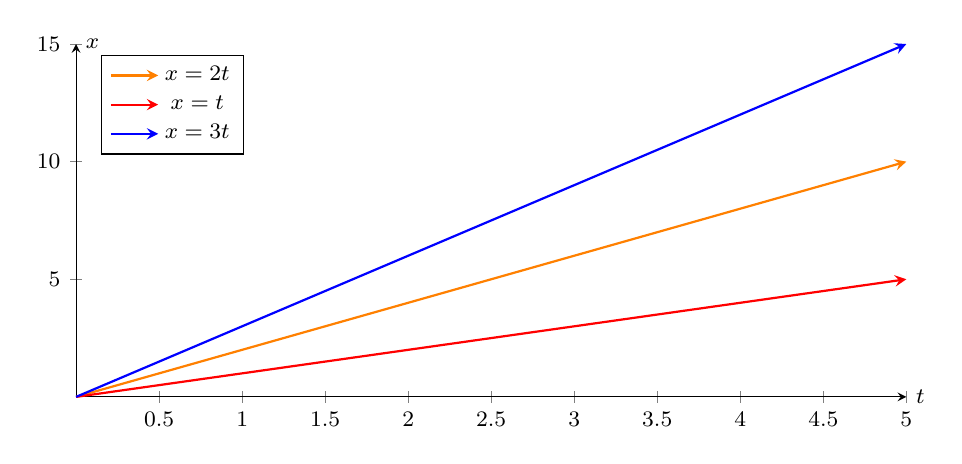
\begin{tikzpicture}
			\begin{axis}[
				my axis style,
				width=\textwidth,
				height=.5\textwidth,
				legend entries={
					$x = 2t$,
					$x = t$,
					$x = 3t$
				},
				legend pos=north west
			]
			
			\addplot[
				domain=0:5,
				thick,
				orange,
				->
			]
			{2*x};
		
			\addplot[
				domain=0:5,
				thick,
				red,
				->
			]
			{(x)};
		
			\addplot[
				domain=0:5,
				thick,
				blue,
				->
			]
			{3*(x)};
			
			\fill[
				black
			];
			
			\end{axis}
		\end{tikzpicture}
		\end{center}
		(continued)
\vspace*{15cm}
\end{soln}
\textbf{\large{1.6 An important note about Calculations}}\\
Unlike mathematics, in physics we care about the units in our calculations. This is because during operations of arithmetic with numbers from physics, we must ensure that the units are compatible. For example, if we are preforming arithmetic with two distance values, we must ensure that they share the same units. When it comes to operations with velocity or acceleration values, then we must ensure that both the [time] units as well as the units of [distance] are compatible.
\newpage 
\begin{ex}
	A racecar clears a $1\km$ track at speed of $500 \m / \s$. Compute the time he took to clear the track in seconds. 
\end{ex}
\begin{soln}
$\implies$
\vspace*{4cm}
\end{soln}



\end{document}
